{ \color{gray}
    --- Move some of this to the introduction, perhaps, or to the chapter on fuzzy spheres. However, I think all what is related to an energy cutoff might be better placed here.
    
    \cite{FioreTheCase2020} Projecting a quantum theory onto the Hilbert subspace of states with energies below a cutoff $\cut E$ may\todo{why may? Do they simply refer to the possibility of this not being a general result?} \rtext{lead to an effective [quantum] theory with modified observables, including noncommutative space(time)}. 
    
        \begin{itemize}
            
        \item Let $S$ be a quantum system with algebra of observables $\acal = \bcal(\hcal)/Lin(\hcal)$ of bounded operators (with dense domain) over the Hilbert space $\hcal$ and hamiltonian $H$. e.g. \lbtext{low-energy effective approximation} of the QM of a system: $\cut \hcal$ is spanned by eigenvectors of energies below a cutoff $\cut E$ e.g. (prototypical example) Peierls projection applied to the Landau model of a charged particle in a plane subject to a perpendicular magnetic field $B$; in that case, if $\cut E = E_0$ the ground state, then $[\cut x_1, \cut x_2] = \frac{i\hbar c}{ie B}$
        
        \item Associated to any (f.d.?) $\cut \hcal \subset \hcal$, its algebra of observables $\lbtext{\cut \acal} := Lin(\cut \hcal)$ satisfies
        \begin{equation*}
            \rtext{\cut \acal = \{ \cut P A \cut P \st A \in \acal\}} 
        \end{equation*}\todo{Is this really true?}\todo{}
        where $\cut P$ is the projection $\cut P : \hcal = \cut \hcal \oplus \cut H^\perp \to \cut \hcal$. 
        
        At least for the low energy effective theories, given an observable $A$, e.g. $A = x_1$ in the Landau model, \rtext{$\cut A$ will measure the SAME PHYSICAL QUANTITY with an uncertantiy compatible with $E \cut E$} here we find the corresponding commutation relations between ``position observables'']\todo{Although I'm not convinced that $\cut x$ is a good alternative version of $x$ in the projected theory, since it involves the action of $x$ itself which involves the creation of high energy eigenstates (), and THEN projecting... but I believe there might be a better notion of position measurement, although I do think that $\cut x$ might be an approximation. D'Andrea \cite{DAndrea2014} might have something to say about this.}
        
        \item If $\cut \hcal$ is such that:
        
            \begin{enumerate}[(i)]
            
            \item $\cut P H = H \cut P$
            
            \item $\cut A$ \todo{is this our case? This } contains all the observables corresponding to measurements that we can \textit{really} perform with the apparati at our disposal.
                
            \end{enumerate}
            
        Then, if the initial state belongs to $\hcal$ / the density matrix belongs to $\cut \acal$ then neither the dynamical evolution (generated by $H$) nor any measurement (due to (ii)) can map it out of $\cut \hcal$, and so \rtext{we can describe the effective theory of $S$ based on $\cut \hcal$, $\cut \acal$ and $\cut H = H|_{\cut \hcal}$}.
        
        \item If $\hcal$ and $H$ (under the induced adjoint action on operators, equivalent to saying that this operator commuts with the group action) are invariant under some group $G$,then so are $\cut P$, $\cut \acal$ (within $\acal$), $\cut H$.
        
        \rtext{Consequence}: if in the complete quantum theory of the system the coordinates $x_i$ commute (``commutative space''), this will not be in true, in general, for the effective theory: $[\cut x_i, \cut x_j] \neq 0$.
        
        \end{itemize}
        
        
        
    \cite{FioreTheCase2020} Adding a confining potential well $V$ with a very sharp minimum on a submanifold $N$ of the original space(time) $M$ may\todo{perhaps here the may refers to whether that is a correct interpretation of what is being done, since it might not be correct to say that we are doing $QM$ on $N$?} \rtext{induce a dimensional reduction to a \textbf{noncommutative quantum theory} on $N$} [the noncommutative quantum theory part, just as in the theory of Chakraborty and Scholtz, seems to mean that not only do the coordinates of phase space commute, but also that the space coordinates themselves do not commute.]
    
    
    Why does it make sense to have an energy cutoff? At least $2$ reasons:
        
            \begin{enumerate}
                
            \item Where neither we nor the environment can bring a state to higher energies. This gives an effective description of the system which is, in principle, sufficient for determining all physical predictions \& is \textbf{simpler to work with}: \cite{FioreTheCase2020} ``yield a simpler low-energy approximation $\cut {\mathcal T}$ of a well-defined quantum theory $\mathcal T$''
            
            \item We might add $\cut E$ as a point where higher energy physics is unknown. MINE: This means that the theory where no cutoff is introduced is not complete, and instead that we have to work with NC space to begin with to come up with a theory for energies above the cutoff.: \cite{FioreTheCase2020}``help in figuring out from the projected theory a new theory valid also at higher energies''
            
            \item \cite{FioreTheCase2020} Regularization procedure of a QFT theory: an energy cutoff $\cut E$ may allow to make sense of the theory if it is originally ill-defined due to UV divergences. More details in the intro of the paper: \cite{2020}``make sense of the original theory $\mathcal T$ if $\cut {\mathcal T}$ is well defined while $\mathcal T$ is not''
                
            \end{enumerate}
            
    \cite{FioreTheCase2020}The following important observations may stem from the same energy cutoff procedure: introducing an energy cutoff $\cut E$ in a quantum theory on a commutative space(time) $M$, i.e. projecting the theory on the Hilbert subspace with energy below $\cut E$, directly induces a \rtext{noncommutative deformation of the latter [the Q. theory]} and \rtext{lower bounds for the space(time) locallyzability}. Moreover, adding a confining potential well $V$ with a very sharp minimum on a submanifold $N$ of $M$ may induce a dimensional \rtext{reduction to a noncommutative quantum theory on $N$} \rtext{\textbf{\Huge [Here the NC Quantum Theory is obtained from the energy cutoff, and that the resulting NC Theory is a NC approximation of Q. Theory on $N$ comes from the sharp potential; this last one is a \textit{dimensional reduction mechanism}!!}} ].
            \begin{enumerate}
            
            \item Regularization introducing energy cutoff was introduced for QED, although not Poincare covariant.
            
            \item DFR: concensus that any mergint of QM and GR should lead to a cutoff of local energy concentration (and an associated lower bound on localization of events). DFR made this more precise, and proposed that \rtext{the bound on the localizability of events could follow from appropriate NC coordinates}. (he cites a recent review: 10)
            
            \end{enumerate}
    
    \lin 
    
    \cite{FioreTheCase2020} First example of NC spacetime: Snyner in [6]: hope that \rtext{nontrivial commutation relations could cure ultraviolet divergences in QFT} But shortly after regularization introducing energy cutoff was introduced for QED, although not Poincare covariant.
    
    
    \lin   
    
    $O(D)$-equivariance/covariance?
    
        \begin{itemize}
            
        \item \rtext{My best guess:} $O(2)$ acts by diffeomorphisms on the NC space.
            
            \begin{itemize}
                
            \item The action of $G$ makes things fall again in $\mathcal H_{\cut E}$, since it even makes an eigenvalue of $H$ fall again into an eigenvalue of $H$ with the same energy.
$\Rightarrow$ $O(2)$ acts on $\mathcal H_{\cut E}$ $\Rightarrow$ $O(2)$ acts on $\mathcal A_{\cut E}$ by inner automorphisms, i.e. \rtext{$O(2)$ acts by diffeomorphisms on the NC space}.    
            \item The time evolution of a ``rotated'' vector is simply given at any time as the rotation of the evolution of the orignal vector. Alternatively, $H^g = H$, so the time evolution of the a rotated vector is given by the same Hamiltonian.
            
            \item The two above things imply that the evolution of a vector in $\mathcal H_{\cut E}$ is given by the same $H$, and that \rtext{this evolution is invariant under $O(2)$}
            
                
            \end{itemize}
            
        \item Why make so much emphasis on ``the commutation relations (satisfied by the algebra generators) are $G$-invariant?'' And what does it even mean? {\tiny It can't be simply that $[A, B]^g = [A^g, B^g]$ since that is trivial to see given that $g$ acts by inner isomorphisms, and so it wouldn't be necessary to say that this is true since the commutation relations and $H$ (and hence) $P_{\cut E}$ are so... \rtext{but I think that's what makes sense since it would mean that the generated algebra is ``the same''}. It can't mean that $[A, B]^g = [A, B]$, since not even for the generators $\cut{x^\pm}$ that is true, since under reflections $\cut L$ does change.
        }  
        
        \item Fiore and Pisacane 2020: ``$O(D)$-covariance of the theory [$\mathcal T$ or $\cut{\mathcal T}$] means that for any orthogonal matrix $g \in O(D)$ there is a unitary transformation $U(g)$ of the [corresponding] Hilbert space $\hcal$ or $\cut \hcal$ such that $g^i_j v_j = U^\dagger(g) v_i U(g)$ for all vectors $\vec v$, and similary for other $O(D)$-tensors''. This, in the $D = 2$ case I have seen this to be satisfies for the $\vec{\cut x}$ observables, in which case it comes the commutation of the projection ($\rightarrow$ of $H$) with the $O(2)$-action.
        
        \item For ``\lbtext{covariance}'': $G$ is a symmetry of the theory:
            
            \begin{itemize}
                
            \item $[g\cdot , H] = 0$ implies \otext{$[g\cdot , P_{\cut E}] = 0$}
            
            \item That, in turn, implies that \otext{$\cut{A}^g = \cut{A^g}$}
                
            \end{itemize}
            
        \end{itemize}
    
    \lin
    
    Results \cite{FioreTheCase2020}:
        \begin{itemize}
        
        \item $\acal_\Lambda$ is a fuzzy approximation of the whole algebra of observables of the particle on $S^d$ (phase space algebra), and converges to the latter in the limit $\Lambda \to \infty$.
        
        \item $\{\mathcal C_\Lambda\}$ can be interpreted as the space of functions on fuzzy configuration space $S^2\Lambda$; while Madore's $\{\acal_\Lambda\}$ should be interpreted only as the space (actually, the algebra) of functions on a \textit{fuzzy spin phase space $S^2_n$}
            
        \end{itemize}
    
    \lin
    
    Applications:
    
        \begin{itemize}
            
        \item \cite{FioreTheCase2020} These models might be suggestive for effective models in quantum field theory, quantum gravity or condense matter physics.
        
        \item Fuzzy spaces:
        
            \begin{itemize}
                
            \item \cite{FioreTheCase2020}As a non-perturbative technique in QFT (orstring, or M-) theory based on finite-discretization of space(time) \textbf{altetnative to the lattice one}: they have the advantage that can carry representations of Lie groups (not only discrete ones)
            
            \item In a \textbf{QFT on a fuzzy space} \textit{the cutoff $n$ works as a parameter regularizing UV divergences}, because integration over fields amounts to integrations over matrices of finite size, growing with $n$ (he cites specific examples.)
            
            
            \item In QFT Enlarging spacetime $M$ by $M' = M \times S_n$ where $S_n$ is a fuzzy space reduces the number of massive Kaluza-Klein modes of a field theory on $M'$.
            
            \item In the matrix model formulations of $M$-theory and string theory, fuzzy spaces may arise as subalgebras giving rise to the leading order of path-integrals over larger matrix algebras
            
            \item Hence $M$-theory they lead to quantized branes in $11$ dimensional spacetime, and in string theory in $10$ dimensional ST.
                
            \end{itemize}
            
        \end{itemize}
}

%%%%%%%%%%%%%%%%%%%%%%%%%%%%%%%%%%%%%%%%%%%%%%%%%%%%%%%%%%%%%%%%
%%%%%%%%%%%%%%%%%%%%%%%%%%%%%%%%%%%%%%%%%%%%%%%%%%%%%%%%%%%%%%%%
\section{General Setting}

% {
%     \color{gray}
    
%     - $H = - \frac{1}{2} \Delta + V(r)$ invariant under $O(D)$
    
%     - Introducing the cutoff $\cut E$, as the energy where
%     \begin{align}
%         \label{eqn5}
%             V(r) \approx V_0 + 2k(r-1)^2 && \text{for $r$ such that $V(r) \leq  \cut E$}.
%     \end{align}
%     %in the region $\nu_{\cut E} = \{r \,|\, V(r) \leq \cut E\}$.
    
%     - Eigenfunctions of $H$ as product of a spherical harmonic $Y(\phi, \dots)$ (eigenvector of $L^2$) and an eigenfunction of the radial equation 
%     \begin{align}
%         \label{eqn9}
%         \left[-\partial_r^2 - (D-1) \frac{1}{r} \partial_r + \frac{1}{r^2} j(j+D-2) + V(r)\right] \tilde f(r) = E \tilde f(r).
%     \end{align}
%     - This last equation can be approximated by a harmonic oscillator equation, since outside the region $\{V(r) \leq \cut E\}$ $\psi$ is negligibly small.
%     : \rtext{$\hcal_{\cut E} \approx $ solutions of Schrodinger Eq. of energy $\leq \cut E$, $\acal_{\cut E} = End(\hcal_{\cut E})$}.
% }

\linea

In dimension $D = d + 1 \in \ZZ_{\geq 2}$, let/the dynamics of a quantum spinless particle with wavefunction $\psi(\vec r) \in \hcal$, where $\hcal = L^2(\RR^D)$ is the Hilbert space of square integrable complex valued functions on $\RR^D$, be/is described by Schr\"odinger equation which, using natural units where $\hbar = c = 1$, looks as follows:
\begin{equation} \label{SchrodingerEquationFullGeneralD}
    H \psi = i \frac{\partial}{\partial t} \psi,
\end{equation}
where $H$ is the Hamiltonian operator of the system
\begin{equation}
    H = -\frac{1}{2} \Delta + V(r);
\end{equation}
here, $\Delta = \sum_{i = 1}^D \frac{\partial}{\partial x^i} =: \sum_{i = 1}^D \partial_i \partial_i$ is the Laplacian of $\RR^D$, where $x^i$, $i = 1, \dots, D$ are the Cartesian coordinates on $\RR^D$. 

The first ingredient to construct the new fuzzy spheres $\{S^d_\Lambda\}_{\Lambda \in \NN}$ is to suppose that the potential is nearly harmonic with minimum value $V(1) = V_0$ at $r = 1$, i.e. that
\begin{align}\label{equationPotentialHarmonicGeneralD}
            V(r) &\approx V_0 + 2k(r-1)^2 & k \geq 0
    \end{align}
in some region $\nu_{\cut E} := \{r \,|\, V(r) \leq \cut E\}$, for some energy value $\cut E \geq V_0$; actually, to obtain simple eigenvalues of the Hamiltonian, $V_0$ will be chosen such that the lowest energy $E$ is $0$, making of $V_0$ a function of $k$. Furthermore, we will suppose that $k = V''(r)/4 > 0$ is very large, so that $V(r)$ is a close to a confining potential for the particle into the $d$-sphere, $S^d$; this condition on $k$ will be made more precise below, when the cutoff energy is introduced.

\lin

As stated in the introduction, we wish to introduce the new fuzzy sphere as the space of observables of the vector subspace of $\hcal$ inside which no wavefunctions of energy higher that some cutoff energy inhabit, hence we need a description of the eigenfunctions of the energy operator, i.e. of the Hamiltonian. 
To do this, we use polar coordinates $r, \phi, \cdots$ where $r = \sqrt{\sum_i (x^i)^2}$ is the radius, and $\phi, \cdots$ are angles on $S^d$, so
\begin{equation}\label{LaplacianPolarCoordinatesGeneralD}
    \Delta = \partial_r^2 + (D-1)\frac{1}{r} \partial_r - \frac{1}{r^2} L^2,
\end{equation}
where, letting $p_i$, $i, j = 1, \dots, D$, be the linear momentum conjugate to $x^i$, and $L_{ij} = i(x^i p_j - x^j p_i)$ be the angular momentum components, then $L^2 = \frac{1}{2} \sum_{i, j} (L_{ij})^2$ is the square angular momentum operator, and also the Laplacian on $S^d$ as the above equation shows. It is well known \cite{} that the eigenvectors of $L^2$, called \dbtext{spherical harmonics}, have eigenvalues $j(j+D-2)$, for $j = $\todo{I think $j \in \ZZ_{\geq 0}$}. 

For the eigenfunction $\psi$ of $H$ with eigenvalue $E$  we may use the ansatz
\begin{equation}\label{ansatzSolutionEigenfunctionEigenvalueEnergyHamiltonianGeneralD}
    \psi(r, \phi, \dots) = \tilde f(r) Y(\phi, \dots).
\end{equation}
Using separation of variables on the Schr\"odinger equation \ref{SchrodingerEquationFullGeneralD} we deduce that \textbf{$\psi$ is an eigenfunction of $L^2$ with eigenvalue $j(j+D-2)$}; this means that we may add a first label $j$ to the observable energy: $E_j$. On the other hand, the radial part of $\psi$ satisfies
\begin{align}\label{equationRadialSchrodingerGeneralDPolarAngles}
        \left[-\partial_r^2 - (D-1) \frac{1}{r} \partial_r + \frac{1}{r^2} j(j+D-2) + V(r)\right] \tilde f(r) = E_j \tilde f(r).
\end{align}

By Fuchs theorem \ref{}, for this equation to have a solution, $V(r)$ needs to grow at most as $\beta/r^2$ when $r$ goes to $0$, for some $\beta \geq 0$ and $\alpha = \sqrt{\beta + j(j+D-2)}$, in which case equation \ref{equationRadialSchrodingerGeneralDPolarAngles} has two independent solutions with asymptotic behavior $r^\alpha$ and $r^{-\alpha}$, respectively, as $r$ goes to $0$. For $\tilde f$ to be defined in the origin the contribution of the second solution must vanish, in particular $\tilde f(0) = 0$; for $\psi = \tilde f\, Y$ to be square integrable on $\RR^D$ it is required that $\tilde f(r) \to 0$ as $r$ goes to infinity.
We now see that the near confining harmonic potential \ref{equationPotentialHarmonicGeneralD} implies that the energy eigenfunction $\psi$ becomes negligibly small outside the $\nu_{\cut E}$ region.
Finally, it can be shown that the above equation can be approximated, for $r \approx 1$, by a harmonic oscillator equation
\begin{equation} \label{harmonicApproximationRadialSolutionGeneralD}
    [- \partial_{\tilde r} + \tilde k_j(\tilde r - \tilde r_{j})^2] f(\tilde r) = \tilde E_j \tilde f(r)
\end{equation} 
for some $\tilde r$ function of $r$, $f(\tilde r) := \tilde f(r)$ and $\tilde k, \tilde r_j$ constants, and, furthermore, that the lowest eigenvalue solutions of equation the Schr\"odinger equation are approximately the solutions of the above harmonic oscillator equation; in particular, at least for the lowest eigenvalue solutions $\psi = \tilde f(r) Y(\phi, \dots)$ of the Schr\"odinger equation, the respective energies will have two labels: a label $j \in \ZZ$ coming from the angular factor $Y(\phi, \dots)$, and a label $n \in \ZZ_{\geq 0}$ coming from the radial part $\tilde f(r)$: $E_{n, j}$. Image taken from \cite{Fiore2018}.

\lin

\begin{figure}[h]
    \centering
    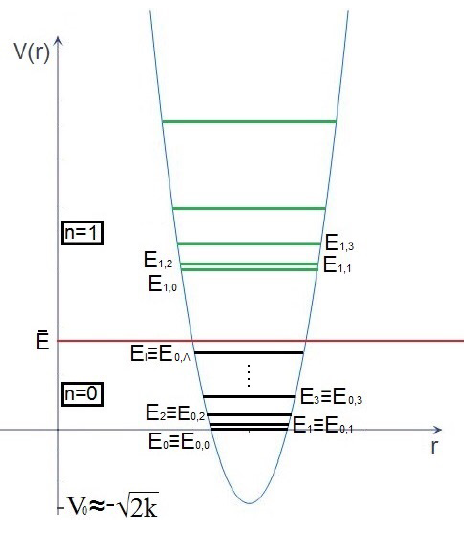
\includegraphics[width = \textwidth/2]{images/FioreEigenvalues.PNG}
    \caption{Eigenvalues of the Hamiltonian for steep enough potential for $D = 2$. The cutoff energy $\cut E$ can be chosen so that the energies below it are the spectrum of the free Hamiltonian $L^2$ in $S^d$.}
    \label{fig:D2EigenvaluesEigenEnergiesHarmonicCutoff}
\end{figure}

As illustrated in \ref{fig:D2EigenvaluesEigenEnergiesHarmonicCutoff}, we will see that, if $\cut E$ is chosen small enough with respect to $k$, e.g. $\cut E \lesssim 8\sqrt{k}$, the eigenvalues of $H$ below $E_{1,0}$ will be a truncation of the spectrum of $L^2$, i.e. the smallest eigenvalues of $H$ will be (approximately) $j(j+D-1)$ for $j = 1, 2, \dots, \Lambda$ for some positive integer $\Lambda$. This introduces the second main ingredient of our construction: \textit{the energy cutoff}. In general, \rtext{for any given $D = d + 1 \in \ZZ_{\geq 2}$, first suppose that $k$ is sufficiently steep to make the eigenvalue $E_{1, 0}$ be above the cutoff energy $\cut E$, %\dbtext{but also that $\cut E$ is high enough so that no eigenvalues are between it and $E_{1, 0}$} 
then, we will define the algebra \lbtext{$\acal_{\cut E}$} as the algebra of operators over the finite dimensional Hilbert space \lbtext{$\hcal_{\cut E}$}, spanned by the solutions $\psi_{0, j} \equiv \psi_j$ of the Schrodinger equation (under the harmonic approximation \ref{harmonicApproximationRadialSolutionGeneralD}) whose energies $E_{0, j} \equiv E_j$ are below $\cut E$}.

In order to make a fuzzy space $\{\acal_\Lambda\}_{\Lambda \in \NN}$ out of this construction of algebras $\acal_{\cut E}$, we need to make $\cut E$ and $k$ grow with a $\Lambda \in \NN$ in such a way that: 1. $k$ is big enough to not produce radial excitations, i.e. keep nontrivial radial eigenfunctions, for which the label $n \geq 1$, above the cutoff; 2. for fixed $\Lambda$, the extremum eigenvalues are $\Lambda(\Lambda + D - 2)$. This may be done, for example, by choosing 
\begin{align}
    \cut E = \cut E(\Lambda) &= \Lambda(\Lambda + d - 1) & k = k(\Lambda) \geq \Lambda^2(\Lambda + 1)^2.
\end{align}

%%%%%%%%%%%%%%%%%%%%%%%%%%%%%%%%%%%%%%%%%%%%%%%%%%%%%%%%%%%%%%%%
%%%%%%%%%%%%%%%%%%%%%%%%%%%%%%%%%%%%%%%%%%%%%%%%%%%%%%%%%%%%%%%%
\section{Construction of $\acal_{\cut E}$ for $D = 2$}

{
    \color{gray}
    
    - Equation \eqref{eqn9} has the approximation, where $\rho := \ln r$
    \begin{equation}
        \label{harmonic2D}
        \hat H f(\rho) = e_m f(\rho), \qquad
        \hat H = - \partial_\rho^2 + k_m(\rho - \tilde \rho_m)^2,
    \end{equation} $
        k_m := 2(k - E'), \quad
        E' := E - V_0, \quad
        \tilde \rho_m := \frac{E'}{k_m}, \quad
        e_m = \frac{E'^2}{k_m} + E' - m^2
    $
    - The solutions $f_{n,m}$ are known, $n \in \bb N, m \in \ZZ$ \then $e_{m, n}(k) = (2n+1)\sqrt{k_m}$ \then $E'_{m,n}(k)$ satisfies a quartic equation \then $E_{m,n}(k, V_0)$.
    
    - Fixing $V_0 = V_0(k)$ such that $E_{0, 0} = 0$ \then $V_0(k) = -\sqrt{2k} + 2 - \frac{7}{2}\frac{1}{\sqrt{2k}} + o(1/k)$ and 
    $\sum_{n = -1}^\infty v_n \left( \sqrt{\frac{1}{k}} \right)^n \approx -\sqrt{2k} + 2 - o(1/k)$ \then
    \begin{equation}
        \rtext{E_{n, m}(k)} = m^2 + 2n\sqrt{2k} - 2n + o(1/\sqrt{k})
    \end{equation}
    
    - Choosing $\cut E < 2 \sqrt{2k} - 2$, the spectrum of $H$ is a truncation of $L^2$: \textbf{the radial oscillations are ``frozen''}: $\cut{\partial_r} = 0$.
    \begin{multline*}
        \lbtext{\psi_m(\rho, \phi)} := f_{0, m}(\rho) e^{im\phi} = c_m e^{im\phi}exp{\left[ -\frac{(\rho - \tilde \rho_m)^2 \sqrt{k_m}}{2} \right]} \\\xrightarrow{k \to \infty} \delta(r-1)e^{i m \phi}
    \end{multline*}
    \begin{equation}
        E = E_m(k) = m^2 + o(1/\sqrt{k})
    \end{equation}
    
    - For $\lbtext{\Lambda} := \lfloor \cut E \rfloor$, 
    \begin{align}
        \lbtext{\hcal_{\Lambda}}:= \lbtext{\hcal_{\cut E}} := span\{\psi_m\}_{|m| \leq 
    \lfloor \cut E \rfloor} ,
    \lbtext{\acal_\Lambda} := \mathcal B(\hcal_\Lambda)
    \end{align}
    
    - Since $H$ generates the time evolution, a
    An element of $\hcal_\Lambda$ doesn't evolve out of $\hcal_\Lambda$.
    
    - Get a fuzzy space: e.g. choosing $k = \Lambda^2(\Lambda+1)^2$ --make $k$ diverge with $\Lambda$ while $\nu_{\cut E}$ goes to $\{r = 1\}$
    
    - This cutoff entails replacing every observable by $A \mapsto \lbtext{\cut A} = P_{\cut E} A P_{\cut E}$% \dbtext{when?}
}

\linea

When decomposing the eigenfunctions of the Schrodinger equation into radial and angular components, $\psi(r, \phi) = \tilde f(r) Y(\phi)$, the angular equation $L^2 Y = EY$ for $D = d+1 = 2$ is 
\begin{equation}
    - \partial_\phi^2 Y = E Y
\end{equation}
since the only angular momentum component is $L_{12} = - L_{21} =: L = -i(x^1 \partial_2  - x_2 \partial_1) = - i \partial_\phi$. The \dbtext{spherical harmonics} are, then, labeled by an integer $m$ and:
\begin{align}
    Y_m(\phi) &= e^{im \phi} & m \in \ZZ\\
    E_m &= m^2.
\end{align}

\lin

Defining $\rho := \ln r$ and $f(\rho) := \tilde f(r)$, the radial equation \ref{equationRadialSchrodingerGeneralDPolarAngles} becomes $f''(\rho) + \{e^{2\rho} [E - V(e^\rho)] - m^2 \} f(\rho) = 0$, and expanding $e^{2\rho}$ about $\rho = 0$ we obtain the following harmonic approximation of the radial equation \ref{equationRadialSchrodingerGeneralDPolarAngles}: 
\begin{equation}\label{equationHarmonicApproximation2DRadial}
        [- \partial_\rho^2 + k_m(\rho - \tilde \rho_m)^2] f(\rho) = e_m f(\rho),\text{ where}
\end{equation}
\begin{equation}\label{equationConstantsHarmonicApproximationRadialD2}
        k_m := 2(k - E'_m),\quad 
        E'_m := E_m - V_0,\quad 
        \tilde \rho_m := \frac{E'_m}{k_m},\quad
        e_m = \frac{E'^2_m}{k_m} + E'_m - m^2.
\end{equation} 
When solving this equation, taking into account that $\psi = f(\rho) $ an additional label $n \in \ZZ_{\geq 0}$ appears to label the eigenvalues of the previous equation; these solutions are:
\begin{eqnsplit}
    f_{n, m}(\rho) &= \exp\{\left[ - \frac{(\rho - \tilde \rho_m \sqrt{k_m})}{2}\right]\} H_n\left[ (\rho - \rho_m)\right]\\
    e_{n, m} &= (2n+1) \sqrt{k_m},
\end{eqnsplit}
where $H_n$ are the Hermite polynomials, $H_n$ being a polynomial of degree $n$ on the dependent variable; in particular, $H_0 = 1$.

From equation \ref{equationConstantsHarmonicApproximationRadialD2} it follows that $E'_m \equiv E'_{n, m} = E_{n, m} - V_0$ satisfies
\begin{equation}\label{equationAlmostQuarticDeterminesE'}
    \frac{E'_{n, m}}{2(k - E'_{n, m})} + E'_{n, m} - m^2 = (2n+1) \sqrt{2(k - E'_{n, m})};
\end{equation}
by squaring both sides we obtain a quartic equation for $E'_{n,m}$ that makes it a function of $k$, and hence we obtain the original eigenvalues of the approximate Schr\"odinger equation $E_{n,m}$ as a functions of $k$ and $V_0$.

\lin

As was mentioned in the previous section, in order to get simple eigenenergies we fix $V_0$ such that the ground energy $E_{0, 0}$ equals $0$. To do this we replace use the tags $m = n = 0$ in equation \ref{equationAlmostQuarticDeterminesE'} and use $E_{0, 0} = 0$. From there, we deduce that $V_0$ has a quartic equation that determines it a function of $k$, which can be rewritten as
\begin{equation}\label{equationV0AlternativeNotQuartic}
    - \sqrt{\frac{1}{2k}}V_0 - \left( \sqrt{\frac{1}{2k}} \right)^3 V_0^2 = \left( 1 + \frac{V_0}{k} \right)^\frac{3}{2}
\end{equation}
. Although a closed formula of $V_0(k)$ is possible, we opt for finding its Taylor expansion with respect to the variable $1/\sqrt{k}$ by using the implicit formula for $V_0(k)$; the resulting formula is:
\begin{equation}\label{equationFormulaExpansionV0functionOfK}
    V_0(k) = - \sqrt{2k} + 2 - \frac{7}{2} \frac{1}{\sqrt{2k}} + o\left(\frac{1}{k}\right).
\end{equation}\todo{check that $o$}
Finally, this expansion in $k$ of $V_0$ induces the following expansion of the eigenenergies of the harmonic approximation of Schrodinger equation:
\begin{equation}\label{equationEigenEnergies2DSchrodingerSolutionsHarmonicApproximation}
    E_{n, m} = m^2 + 2n\sqrt{2k} - 2n + o\left(\frac{1}{\sqrt{k}}\right).
\end{equation}

\lin 

The final step to build the Hilbert space $\hcal_{\cut E}$ and $\acal_{\cut E}$ given a cutoff energy $\cut E \geq 0$, is to make sure that $k$ is steep enough to ensure that $E_{1, 0}$ is above it, and for this is expressed by the inequality
\begin{align}
    \cut E < E_{1, 0} \approx 2 \sqrt{2k} - 2.
\end{align}\todo{perhaps the $o(1/\sqrt{k})$ term is negative?}
In that case, renaming $\psi_{0, m}$ and $E_{0, m}$ as $\psi_m$ and $E_m$ for $m \in \ZZ$, we define the spaces
\begin{eqnsplit} \label{equationDefinitionOFHandEHilbertAndAlgebraGivenCutoff}
    \hcal_{\cut E} &:= span\{ \psi_m(\rho, \phi) \,:\, E_m \leq \cut E \}\\
    \acal_{\cut E} &:= End(\hcal_{\cut E});
\end{eqnsplit} where
\begin{equation}\label{equationDefinitionPsimD2BasisOfHCutE}
    \psi_m(\rho, \phi) = c_m e^{im\phi} \exp \left[ - \frac{(\rho - \tilde \rho_m) \sqrt{k_m}}{2} \right], \quad \text{where}
\end{equation}
\begin{align}\label{equationExpansionKDependentConstantsPsim}
    k_m &= 2k \left( 1 - \frac{2}{\sqrt{2k}} + \frac{2-m^2}{k} + o\left( \frac{1}{k^{3/2}} \right) \right), &
    \tilde \rho_m &= \frac{1}{\sqrt{2k}} + \frac{m^2}{2k} + o\left( \frac{1}{k^{3/2}} \right).
\end{align}

Notice that, in principle, the definition of $\acal_{\cut E}$ is dependent on the chosen $k$ due to $k_m$ and $\tilde \rho_m$, so we may write instead $\psi_{n, m}(\rho, \phi)$ as $\psi_{n, m}(\rho, \phi; k)$; also notice that, for a fixed $k$ and two cutoffs $\cut E_1$ and $\cut E_2 > \cut E_1$ compatible with this $k$, then $\hcal_{\cut E_1}$ is, strictly, a subspace of $\hcal_{\cut E_2}$ since its basis elements $\psi_m$ are also basis elements of the latter, but only due to the fixed choice of $k$ for both cutoffs. 
However, first notice since $k$ is chosen large, all $\psi_m$ essentially vanish outside the $k$ dependent region $\nu_{\cut E}$, for $m$ fixed, and in fact $\psi_m(\rho, \phi) \to e^{im\phi} \delta(\rho - 1)$ in probability as $k \to \infty$; more importantly, the dependence on $k$ of the definition of $\acal_{\cut E}$ will not be relevant to our studies, since all what we will need in order to study the fuzzy spaces they form are the fact that they are endomorphism algebras over finite dimensional Hilbert spaces, and their behavior under the action of the group $O(2)$ induced by the action on the underlying Hilbert space. In fact, it is easy to see (since $O(2)$ doesn't affect the radial coordinate) that, for any compatible $k$, $\hcal_{\cut E}$ is isomorphic to  $\hcal'_{\cut E} := span\{e^{i m \phi} \, : \, m \in \ZZ, \, m^2 \leq \cut E\}$ in an $O(2)$-equivariant way, and, hence, that \rtext{$\acal_{\cut E}$\todo{again, strictly speaking, I am assuming that the extra factor in the $k$-expansion of the energies is positive} is isomorphic to $\acal'_{\cut E} := End(\hcal'_{\cut E})$ as a $C^*$-algebra and as a representation space of $O(2)$}.


Now, to parametrize these algebras by $\Lambda \in \NN$, define
\begin{eqnsplit}
    \hcal_\lambda &:= \hcal_{\Lambda = \lfloor \cut E \rfloor} \\
    \acal_\Lambda &:= End(\hcal_\Lambda);
\end{eqnsplit}
this means that the energies of the basis elements of $\hcal_\Lambda$ are all those $m^2$ that are below the energies $E_{1,0}$. Strictly speaking, to define each $\acal_\Lambda$ we also need to choose $k$ as a function on $\Lambda$ in such a way that it diverges with $\Lambda$ and that $k(N)$ is compatible with the cutoff energy $\Lambda$, for this,  equation \eqref{ } tells us that we can choose any function
\begin{equation}
    k(\Lambda) \geq \Lambda^2 (\Lambda + 1^2).
\end{equation}


%%%%%%%%%%%%%%%%%%%%%%%%%%%%%%%%%%%%%%%%%%%%%%%%%%%%%%%%%%%%%%%%
%%%%%%%%%%%%%%%%%%%%%%%%%%%%%%%%%%%%%%%%%%%%%%%%%%%%%%%%%%%%%%%%
\section{Important Observables and their Commutation Relations}

{
    \color{gray}
    
    - Up to infinite, $1/k^{1/2}\dbtext{?}$ and $1/k^{3/2}$ orders, respectively
    \begin{align}
    \label{projObs2D}
        \rtext{\cut L} \psi_m &= m \psi_m; & 
        \rtext{\cut H} &= \cut L^2; & 
        \rtext{\cut x^\pm} \psi_m = 
            \begin{cases}
                \frac{a}{\sqrt{2}} \sqrt{ 1 + \frac{m(m \pm 1)}{k} } \psi_{m \pm 1} & -\Lambda \leq \pm m \leq \Lambda - 1 \\
                0 & \text{otherwise}
            \end{cases}
    \end{align}
    - And so, up to terms of $1/k^{3/2}$
    \begin{align}
        \label{conmObs2D}
        \cut{x^+}^\dagger &= \cut{x^-}; &
        [\cut L, \cut{x^\pm}] &= \pm \cut{x^\pm}; &
        \rtext{[\cut{x^+}, \cut{x^-}]} &= - \frac{\cut L}{k} + \left[1 + \frac{\Lambda(\Lambda+1)}{k}\right] (\tilde P_{\Lambda} - P_{-\Lambda})a^2.
    \end{align}
     - If \eqref{projObs2D} are used exactly to define elements of $\mathcal B(\hcal_\Lambda) \equiv \acal_\Lambda$ then \eqref{conmObs2D} are also exact, and $\cut{x^\pm}$ generate $\acal_\Lambda$. -- $\cut{\partial_\pm}$ are now redundant... but I'm not sure why
     
}

\linea


%%%%%%%%%%%%%%%%%%%%%%%%%%%%%%%%%%%%%%%%%%%%%%%%%%%%%%%%%%%%%%%%
%%%%%%%%%%%%%%%%%%%%%%%%%%%%%%%%%%%%%%%%%%%%%%%%%%%%%%%%%%%%%%%%
\section{Realization of $\acal_\Lambda$ through $U\soth$}

{
    \color{gray}
    
    - $O(2)$ acts on $\hcal_\Lambda \subset L^2(\RR^2)$, and so \rtext{on $\acal_\Lambda$}, since $[H, O(2)\cdot ] = 0$. through the action induced in $\acal_\Lambda$ by its action on $\RR^2$.
        \begin{itemize}
            
        \item \textit{Rotation} $R_\theta$: $\cut{x^\pm} \mapsto e^{\pm i \theta} \cut{x ^\pm}; \cut L \mapsto \cut L \in \acal_\Lambda$.
        
        \item \textit{Reflection}: $\cut{x^\pm} \mapsto -\cut{x^\mp}; \cut L \mapsto -\cut L$.
        
        \end{itemize}
    
    - \rtext{We can consider \otext{$\acal_\Lambda \cong  M_N(\CC) = \pi_\Lambda(Uso(3))$} \textbf{as a $*$-algebra and representations of $O(2)$}}, where $\pi_\Lambda$ is the $\lbtext{N} := 2 \Lambda + 1$ dimensional representation. $SU(N) \ni g$ is the group of $*$-automorphisms of $M_N(\CC) \cong \acal_\Lambda$ acting by $a \mapsto g a g^{-1}$; $O(2)$ is then a subgroup. Comes from mapping:
    \begin{align}
        \rtext{\cut{x^\pm}} &\longleftrightarrow \rtext{f_\pm (J^0) J^\pm}, &
        \rtext{\cut L }& \rtext{\longleftrightarrow J^0}
    \end{align}
    where $J^\pm, J^0$ is the Weyl-Cartan basis of $so(3)$, $\lbtext{f_\pm(s)} := \frac{1}{\sqrt{2}} \sqrt{\frac{1 + s(s-1)/k}{\Lambda (\Lambda + 1) - s(s-1)}} =: \lbtext{f_-(-s)}$%: $[J^+, J^-] = J^0; [J^\pm, J^0] = \pm J^\pm$

    - $O(2) \subset SO(3)$: \textit{Rotation}: $\pi_\Lambda(e^{i \theta J_0})$; \textit{Refl.}: $\pi_\Lambda(e^{i\pi (J^+ + J^-)/\sqrt{2}})$
    
    \lin 
    
    Let $(V_l, \pi_l)$ be the irreducible representations of $O(3)$ characterized by $L^2 = l(+1)$
    
        \begin{itemize}
        
        \item  \begin{equation}
            \hcal_\Lambda \cong \bigoplus_{l = 0}^\Lambda V_l
        \end{equation}
        
        \item \begin{equation}
            C_\Lambda \cong \bigoplus_{l = 0}^{2\Lambda} V_l
        \end{equation}
        
        \end{itemize}
        
    \rtext{\textbf{As $\Lambda \to \infty$ these respectively become the decomposition of $L^2(S^2)$ \& of $C(S^2)$ that acts on $L^2(S^2)$.}}
}

\linea


%%%%%%%%%%%%%%%%%%%%%%%%%%%%%%%%%%%%%%%%%%%%%%%%%%%%%%%%%%%%%%%%
%%%%%%%%%%%%%%%%%%%%%%%%%%%%%%%%%%%%%%%%%%%%%%%%%%%%%%%%%%%%%%%%
\section{Convergence}

{
    \color{gray}
    
    - \textbf{$\psi_m$ as fuzzy analogues of $e^{i m \phi} \in \hcal$}: $O(2)$-covariant embedding $\hcal_\Lambda \hookrightarrow \otext{\hcal = L^2(S^1)}$, $\psi_m \mapsto e^{im\phi}$; \hfill \\then $\hcal_\Lambda \to \hcal$ as $\Lambda \to \infty$ in the sense that $\forall \phi \in \hcal$, $\lbtext{\phi_\Lambda} := \sum_{|m| \leq \Lambda} \phi_m e^{im\phi} \to \phi$ in the $L^2$-norm.
    
    - Induces, \rtext{embedding $\acal_\Lambda \hookrightarrow \otext{\acal = \mathcal B(\hcal)}$ and limit $\acal_\Lambda \to \acal$} as $\Lambda \to \infty$.
    
    - \textbf{Fuzzy analogue of $B(S^1)$ of (bounded) functions on $S^1$} as subalgebra (act by mult.) of $\mathcal B(\hcal)$: $\lbtext{C_\Lambda} := \left\{ \sum_{h = -2\Lambda}^\Lambda f_h \eta^h \,|\, f_h \in \CC\right\}$ where $\eta^\pm  = \frac{\sqrt{2}}{a}x^\pm$ (so $\eta^\pm \to e^{\pm i \phi}$ as operators).
    
    - Choosing $k(\Lambda) \geq 2 \Lambda(\Lambda + 1)(w\Lambda+1)^2$, then \rtext{$B(S^1) \to \mathcal B(\hcal)$ as operators} due to the strong limits: $\hat f_\Lambda \to f\cdot$, $\hat{(fg)}_\Lambda \to fg\cdot $, $\hat f_\Lambda \hat g_\Lambda \to fg\cdot$, where $\lbtext{\hat f_\Lambda} := \sum_{h = -2\Lambda}^{2\Lambda} f_h \eta^h$ is ``truncation'' of $f \in B(S^1)$.
    
}

\linea

